\section{Results}

\def\figwidth{0.9\textwidth}

We successfully deployed a service that provides an up-to-date search interface. We are spread across Azure, AWS, and Vercel. The service is available at \url{https://doyenapp.org}, available for all to use.

\subsection{Our Data}

We were able to implement a robust and replicable deployment for our Elasticsearch instance using AWS and CloudFormation. CloudFormation encapsulates our cloud infrastructure in code so that the details which often hinder the replication of infrastructure are already accounted for. We were able to index 8.7 million PubMed articles, all from the last 10 years. It takes 4.5 hours to load the content from PubMed into our Elasticsearch instance. We have set up an automatic update for the content that will run weekly.

We deployed an API on Azure which serves our data to the user interface. Here we have implemented the ability to filter by our custom Expert Score based on the document relevancy score, the number of publications for each author, and the overall citation count. We implemented a filter by the time range of publication, although that is not yet exposed in the user interface. Requests to the API return hundreds of results in mere seconds.

\subsection{User Interface}

To make the application easy to use, we created a responsive browser application that can be accessed anywhere with internet access. The app allows users to enter MeSH terms or general keywords, as shown in \autoref{fig:ui-main}. Users can access an autocomplete dropdown list of MeSH terms for ease of discovery. They can populate the search bar with multiple terms, with the additional ability to refine the search by adding and removing search terms. When users are satisfied with their staged query and hit "search," the search terms list is sent to Elsaticsearch for a quick search of indexed PubMed publications. A key advantage of Elasticsearch is that we can search for any term in publication abstracts and titles and are not restricted to MeSH terms. Elasticsearch results are then displayed in an interactive table for users to refine and filter as they see fit. They initially see the top 50 results sorted by the highest Relevancy Score. However, they can quickly sort the table based on the Relevant Publication count and Relevant Citation count and filter by the number of each. Experts containing author identification displays an additional dropdown for users to view a list of co-authors who have worked with the expert listed. Finally, users can click to view the same publications that are relevant to the search used.

\begin{figure*}[ht!]
    \tiny
    \centering
    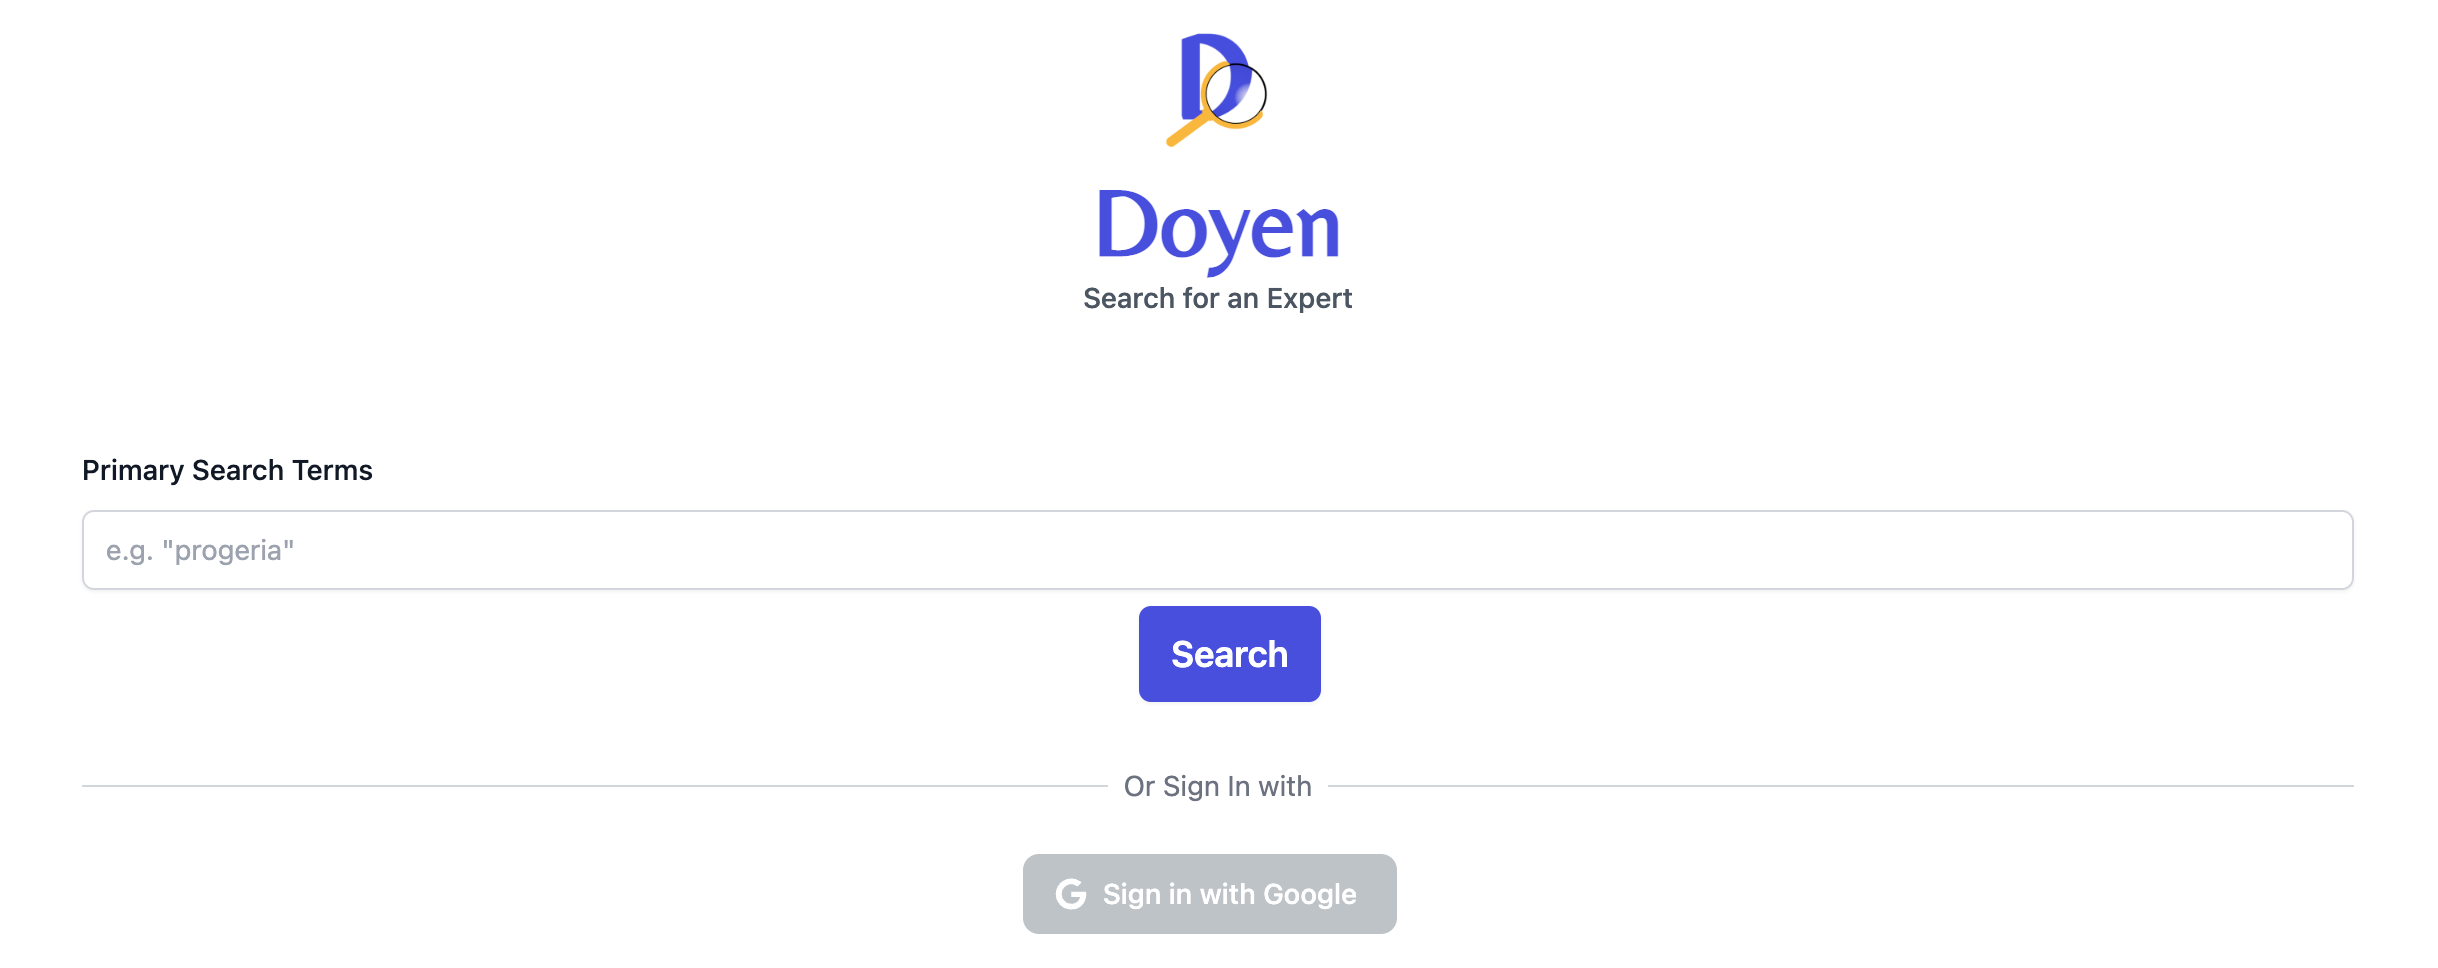
\includegraphics[width=\figwidth]{Images/ui-main.png}
    \caption[Doyen app home page]{\textbf{Doyen app home page:} A view of the landing page for the Doyen app, with the search bar and sign-in options}
    \label{fig:ui-main}
\end{figure*}

The autocomplete dropdown, shown in \autoref{fig:ui-auto-dropdown} list is populated with over 60,000 MeSH terms sourced from PubMed, providing users with a comprehensive set of keywords for query construction. Users can select desired terms from the dropdown list, which are then used to build a keyword query in the search bar. The query can be easily modified by adding or removing keywords before submission, initiated by clicking the "Search" button.
\begin{figure*}[hb!]
    \tiny
    \centering
    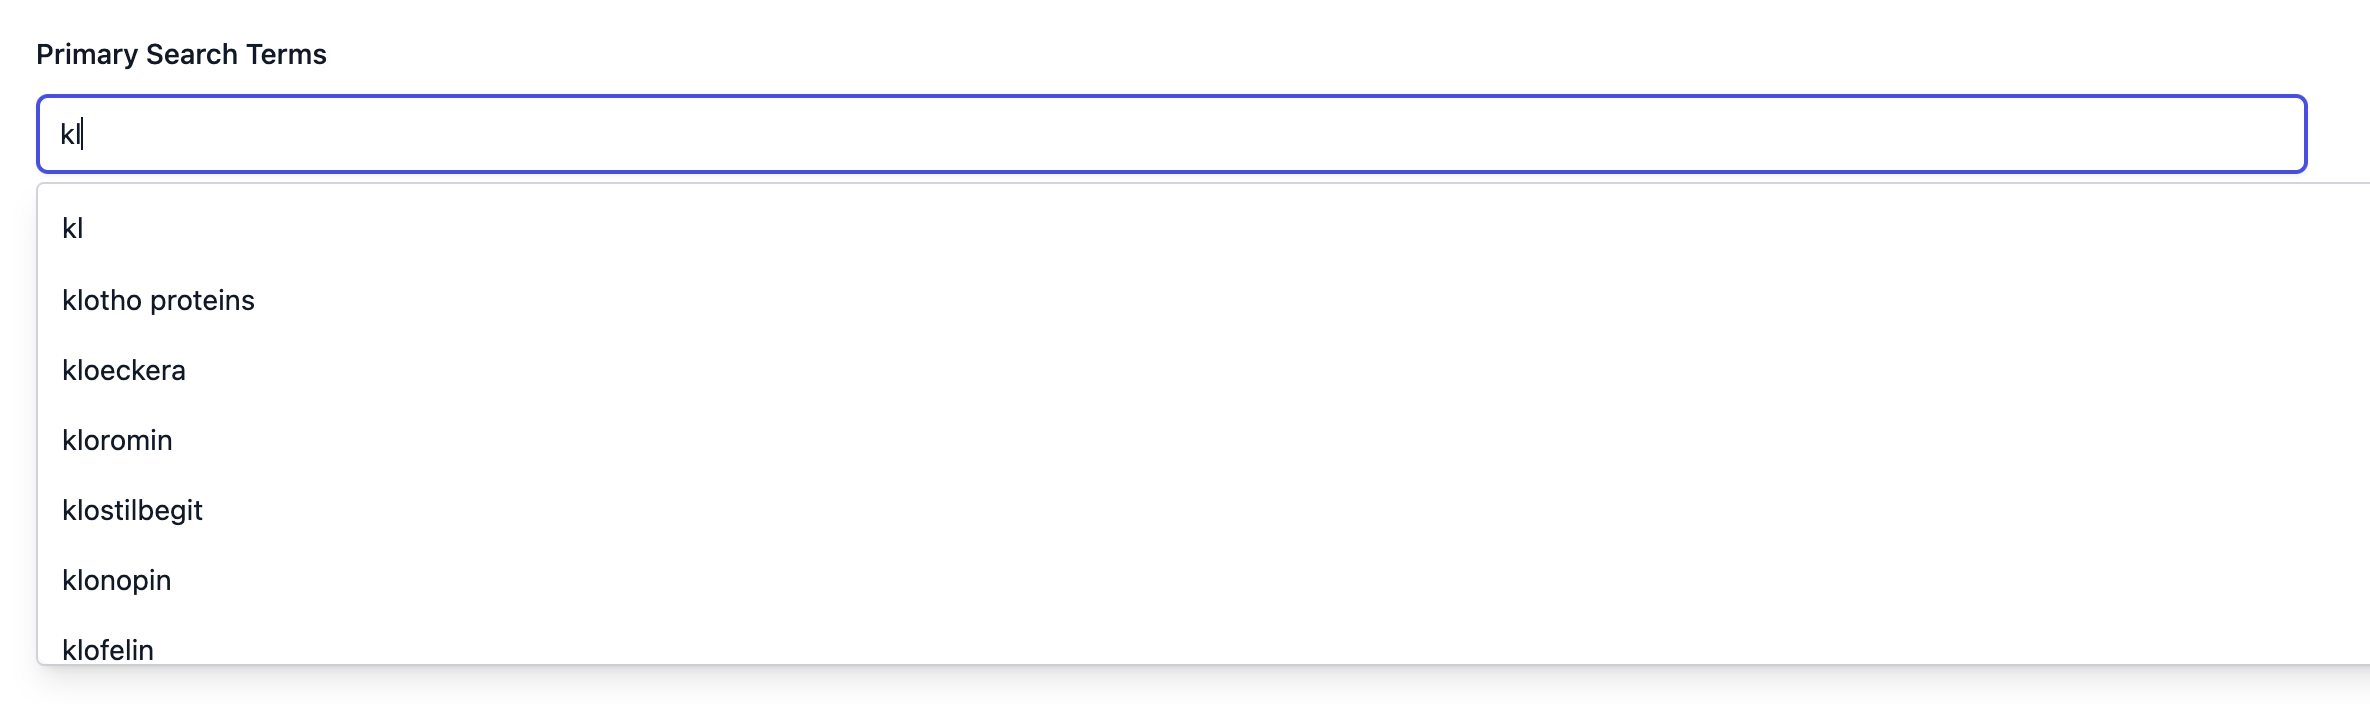
\includegraphics[width=\figwidth]{Images/ui-autocomplete.png}
    \caption{Search autocomplete dropdown}
    \label{fig:ui-auto-dropdown}
\end{figure*}

\subsubsection{Side Panel Filters and MeSH Term Hierarchy}

The expandable side panel, shown in \autoref{fig:ui-search-query}, allows users to refine their search query further by applying filters based on publication dates, author expertise, and institution type. Additionally, the side panel features a clickable MeSH term hierarchy, enabling users to delve deeper into the MeSH term tree and perform more targeted searches.
\begin{figure*}[hb!]
    \centering
    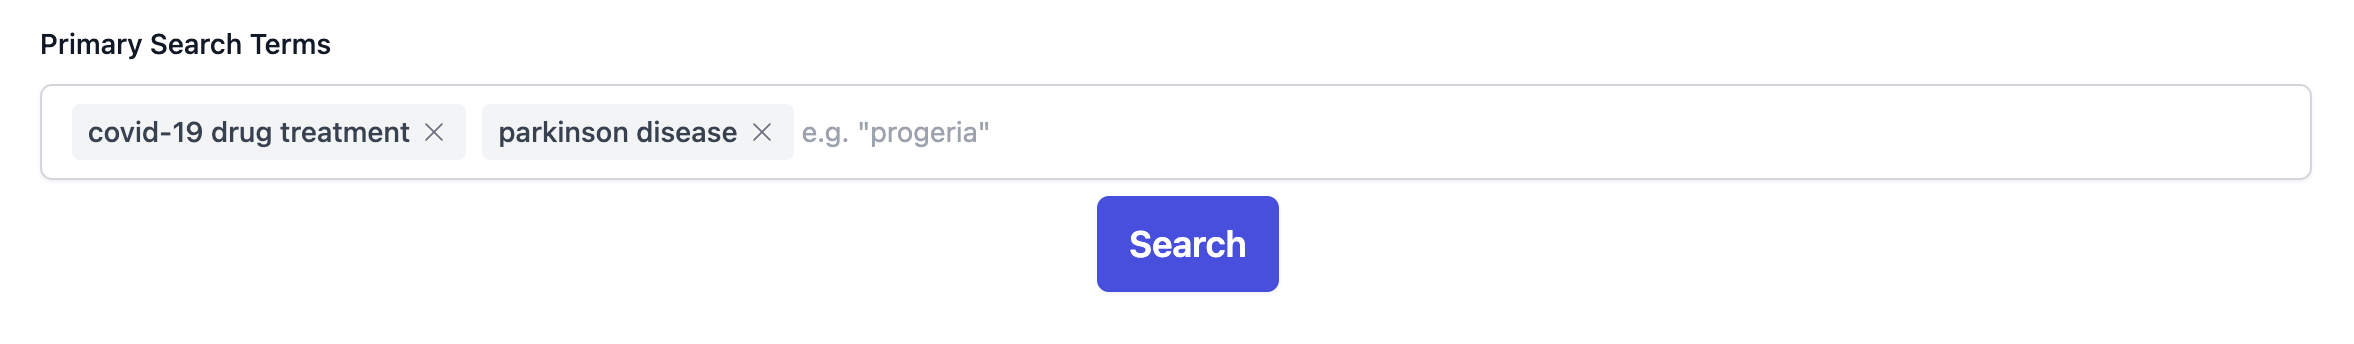
\includegraphics[width=\figwidth]{Images/ui-query.png}
    \caption{Build a search query}
    \label{fig:ui-search-query}
\end{figure*}

\subsubsection{Backend Integration and Search Results Display}

Users can download a PDF list of all returned authors for future reference or investigate specific authors further by clicking on their information cards. This functionality, shown in \autoref{fig:ui-results} allows users to access and explore pertinent information efficiently, enhancing the overall search experience provided by our web application.
\begin{figure*}[ht!]
    \centering
    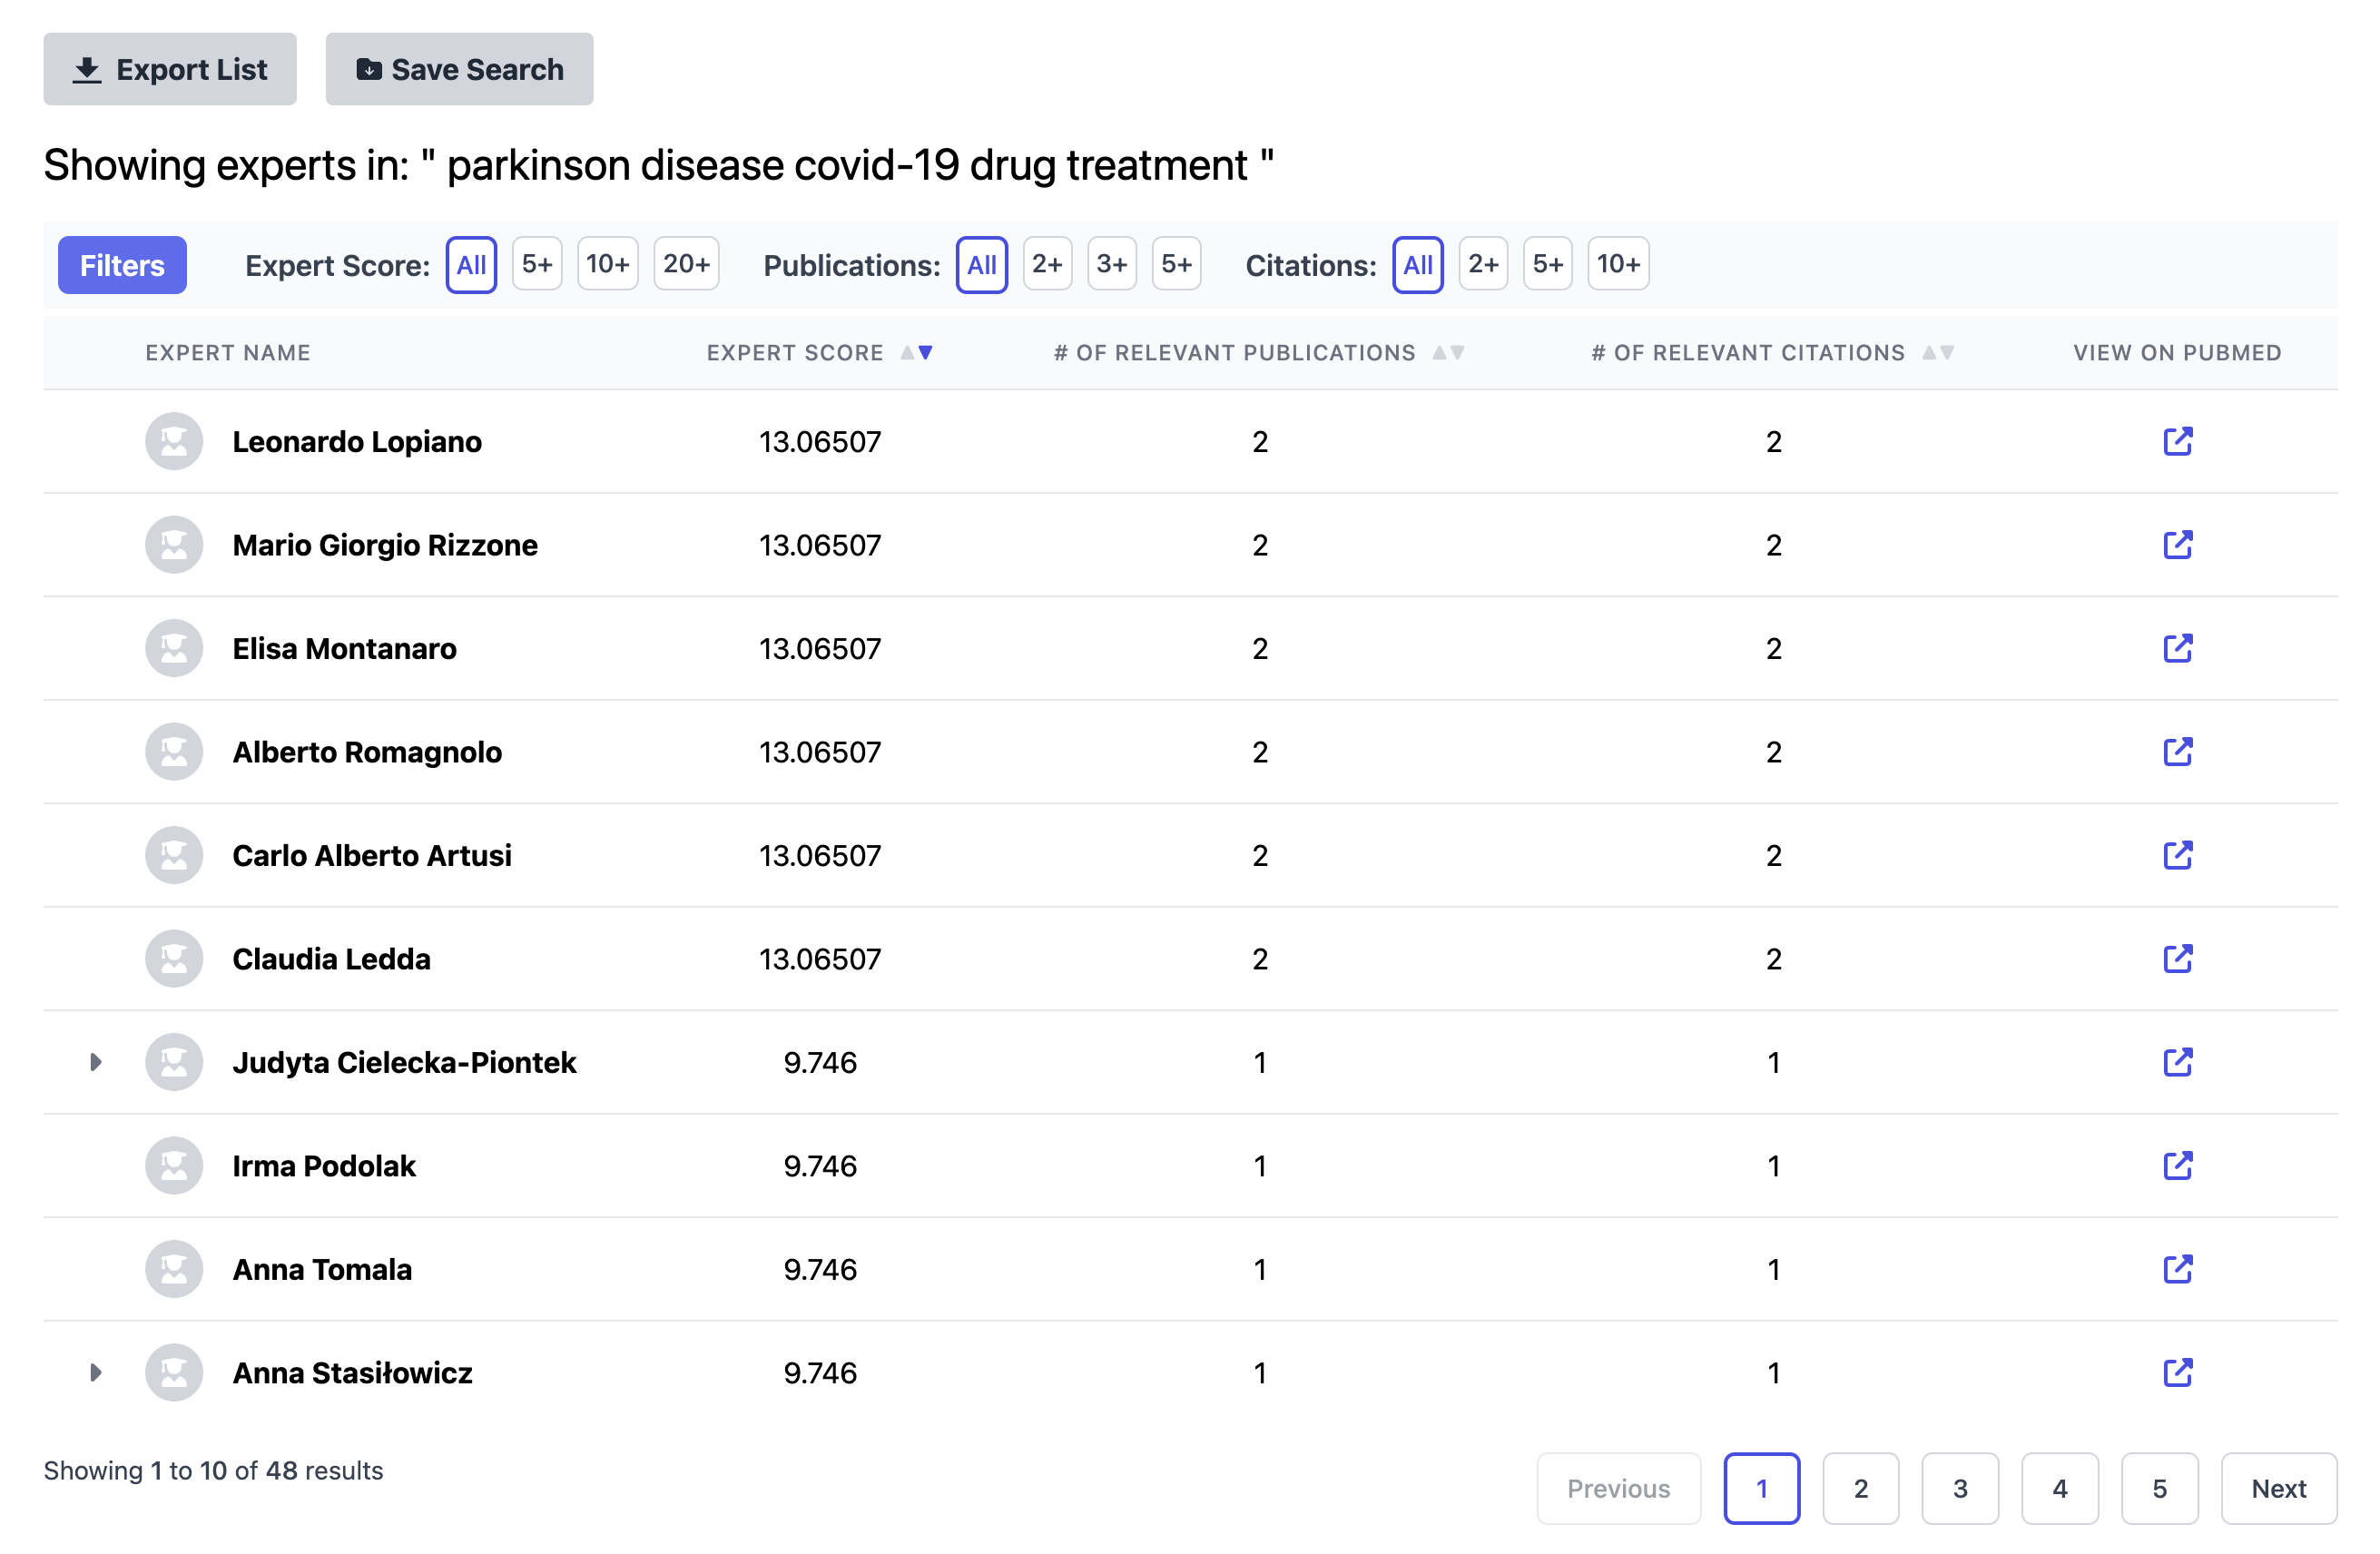
\includegraphics[width=\figwidth]{Images/ui-results.png}
    \caption{Results page from user query}
    \label{fig:ui-results}
\end{figure*}

As shown in \autoref{fig:ui-co-author-dropdown}, upon submitting a search query, the web application sends an API request to the backend, which processes the query and returns a JSON object containing relevant search results. These results are then displayed on the results page, giving users an overview of the returned authors and their associated information.
\begin{figure*}[hb!]
    \centering
    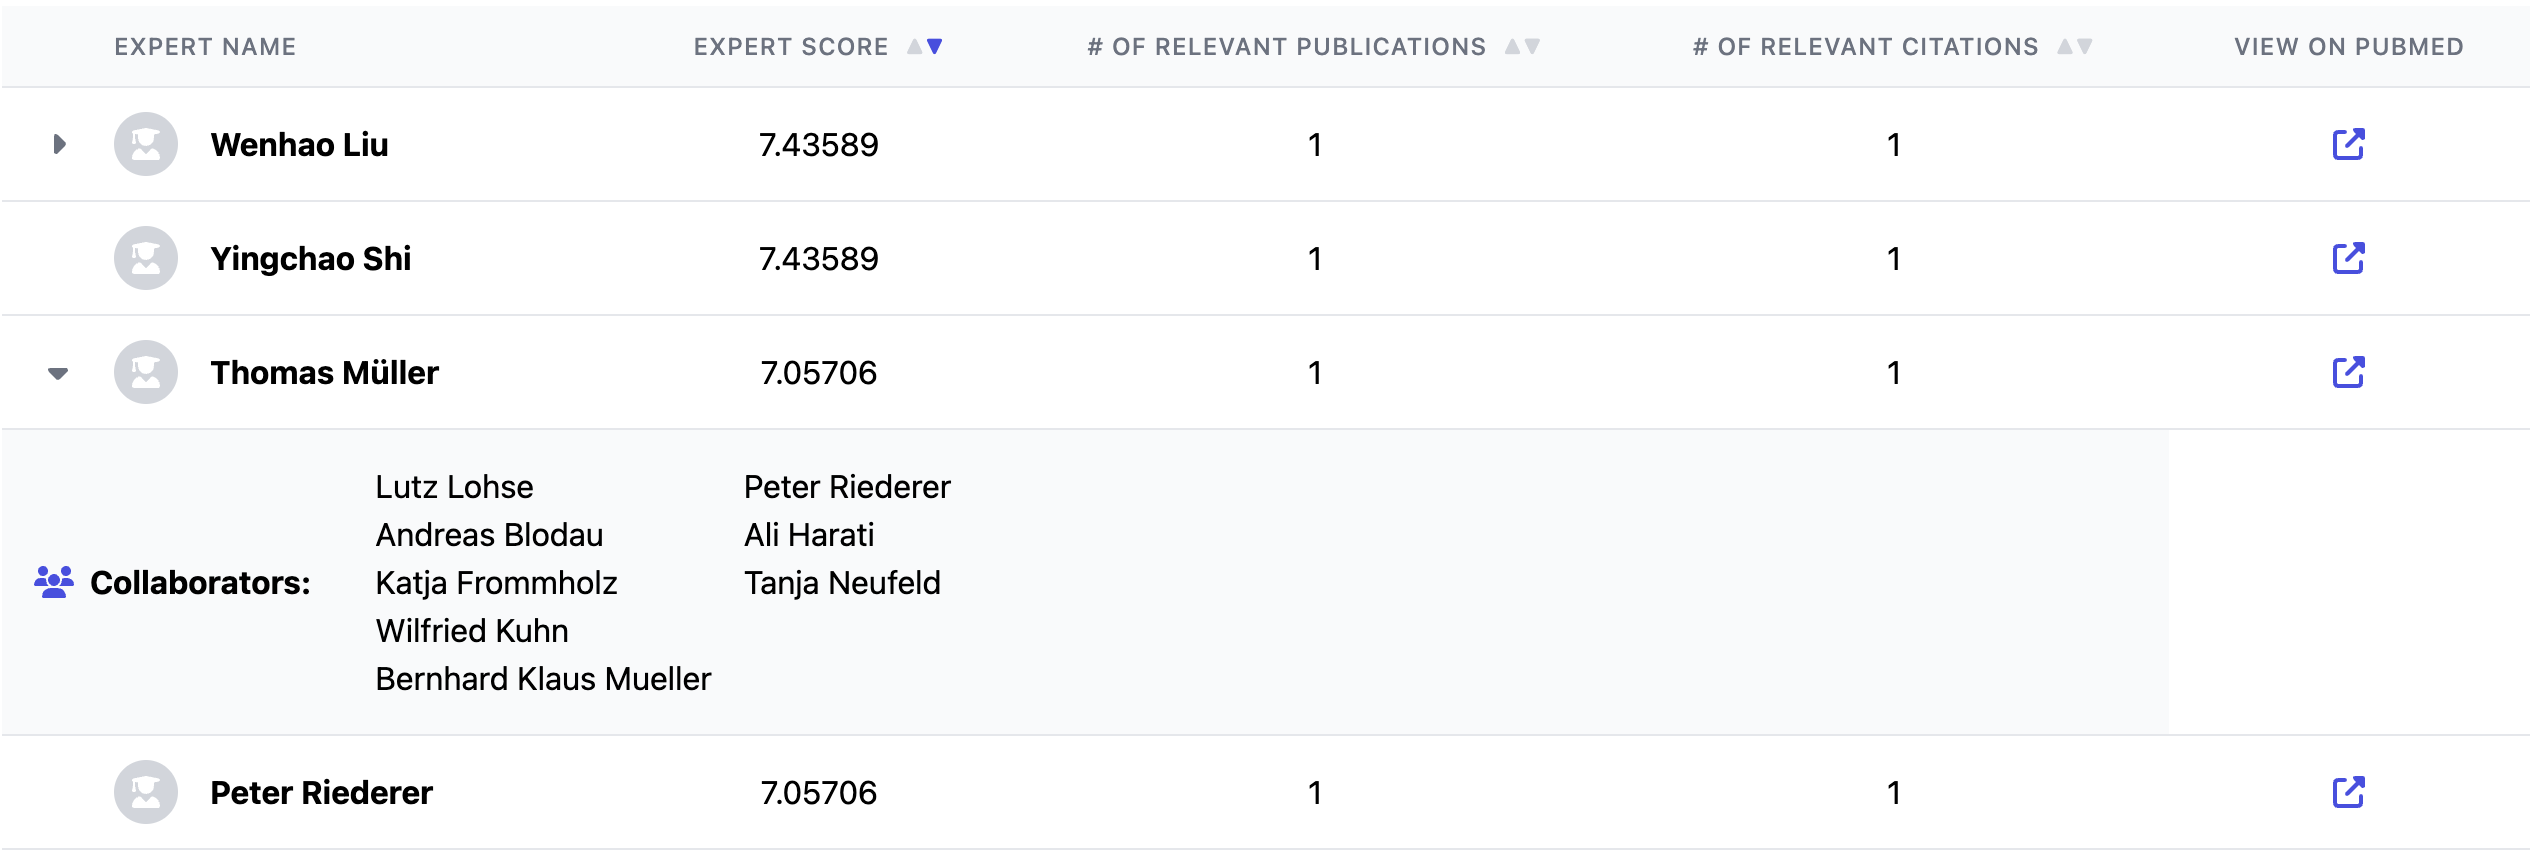
\includegraphics[width=\figwidth]{Images/ui-author-card.png}
    \caption{Expert co-author dropdown list}
    \label{fig:ui-co-author-dropdown}
\end{figure*}
